\chapter{Experiments}
\label{sec:experiments}

Our final dataset for training the triplet loss model consisted of 20000 triplets, gradually accumulated through our labeling application. We employed consistent training configurations (\autoref{sec:training-setups}). The experiments were conducted using two different model architectures : GNN (\autoref{sec:graph-based-models}) and Transformer-based models (\autoref{sec:transformer-based-models}). 

\section{Training setups}
\label{sec:training-setups}

\subsection{Data}

The dataset used for training the models consists of 20000 triplets, each containing three 3D designs: an anchor, a positive, and a negative model. Input data are meshes stored in stl files.

For the GNN model, vertices of the mesh are represented as nodes in a graph, while edges are defined based on the connectivity of the vertices. When two vertices share a face, an edge is created between them. 
For the transformer model, that take as input a point cloud, we convert the mesh into a point cloud by sampling points uniformly from the surface of the mesh. The number of sampled points is fixed to 10000, following \cite{liuOpenShapeScaling3D2023}.

Initially, the use of Principal Component Analysis (PCA) for training or inference, as done in \cite{popRotationInvariantGraph2023}, was considered but ultimately discarded. The idea of PCA is appealing because it allows working within a canonical reference frame. However, to ensure the model is as general as possible, data augmentation techniques were favored over PCA. One of the issues with PCA is demonstrated in \autoref{fig:pca_problem}. Additionally, we prefer to let the model architecture handle these aspects directly.

\begin{figure}[]
    \centering
    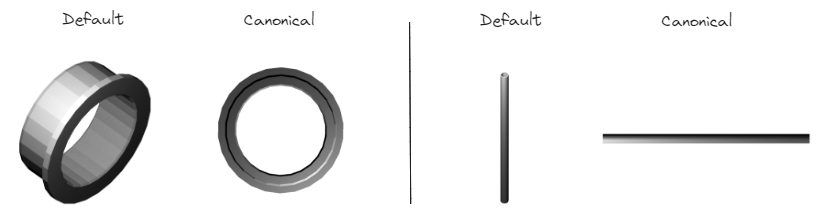
\includegraphics[width=\columnwidth]{images/pca_problem.png}
    \caption{Illustration of the issue using PCA as a preprocessing step. Both designs are tubular structures, shown in their default orientation and in the canonical reference frame. While the design on the left aligns its first principal axis with the tube's axis, the design on the right does not. This inconsistency can result in misalignment during training, particularly since the behavior varies depending on the specific design.}
    \label{fig:pca_problem}
\end{figure}

Data augmentation was performed to enhance the model's robustness, especially considering rotations. Other augmentation techniques, such as symmetry and noise addition, were also explored but ultimately discarded. The following two techniques were retained:
\begin{enumerate}
    \item \textbf{Normalization to unit sphere}: We standardize all the designs to fit within a unit sphere. This enhances the model's ability to capture geometric features rather than scale. The length of the design has been integrated into the architecture of the GNN model.
    \item \textbf{Random rotations}: Each design is randomly rotated around the three axes. This is crucial for ensuring that the model learns to recognize designs regardless of their orientation. A special focus was placed on rotation invariance, as explained hereafter.
\end{enumerate}

Rotation invariance is a critical aspect of our model, as it allows the model to recognize designs regardless of their orientation. This is particularly important in our context since 3D designs designers often work with similar designs saved in different orientations. To achieve this, 3 metrics were defined to evaluate the model's performance in terms of rotation invariance:
\begin{itemize}
    \item \textbf{Mean distance to rotated distribution}: This metric calculates the average distance between the model's prediction of a design and the predictions of its $n$ rotated versions. 
    \item \textbf{Median distance to rotated distribution}: Similar to the mean distance, this metric computes the median distance between the model's prediction and the predictions of the $n$ rotated versions.
    \item \textbf{Rotation matching accuracy}: The two previous metrics are absolute. To provide a more relative measure, we also compute a rotation matching accuracy. If we fix a value of $n$, we can compute the proportion of nearest neighbors in the whole dataset that are also among the $n$ rotated versions of the design. $n$ is set to 10 in our experiments, as for the two previous metrics.
\end{itemize}

Initially, data augmentation was performed offline. This means that for each triplet, each design was augmented by applying random rotations before the training process. We choose 10 rotations per design, as it yields the best results as shown in \autoref{fig:rotated_study}. Results are shown with our starting GNN EdgeConv model.
\begin{figure}[]
    \begin{subfigure}[h]{0.5\linewidth}
        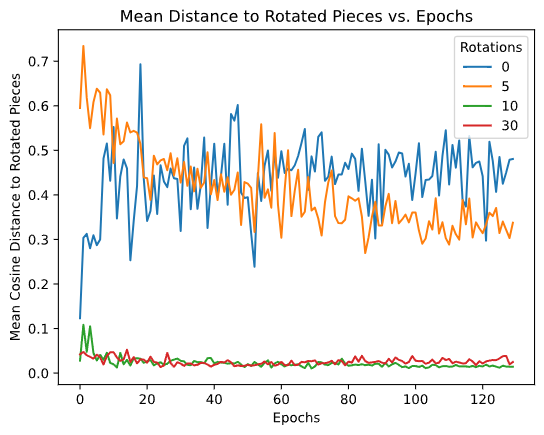
\includegraphics[width=\columnwidth]{images/mean_rotated_study.png}
        \caption{Mean distance to rotated distribution.}
        \label{fig:mean_rotated_study}
    \end{subfigure}
    \hfill
    \begin{subfigure}[h]{0.5\linewidth}
        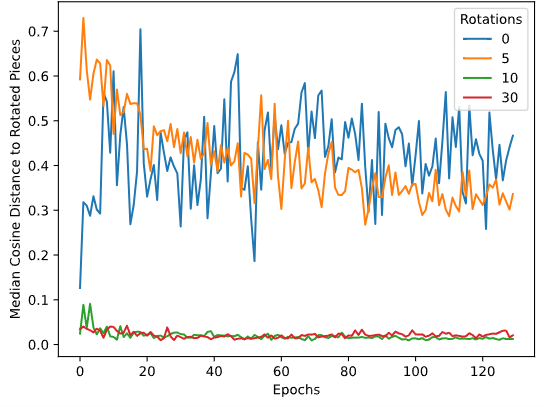
\includegraphics[width=\columnwidth]{images/median_rotated_study.png}
        \caption{Median distance to rotated distribution.}
        \label{fig:median_rotated_study}
    \end{subfigure}
    \caption{Influence of the number of rotations on the rotations metrics.}
    \label{fig:rotated_study}
\end{figure}

We also experienced online data augmentation, where random rotations are applied on-the-fly during training. Indeed, there is no clear recipe for the best approach \cite{OfflineDataAugmentation} and we wanted to explore both options. The results of both approaches are compared in \autoref{fig:augmented_data_comparison}. The offline augmentation approach yielded better results.
\begin{figure}[]
    \begin{subfigure}[h]{0.5\linewidth}
        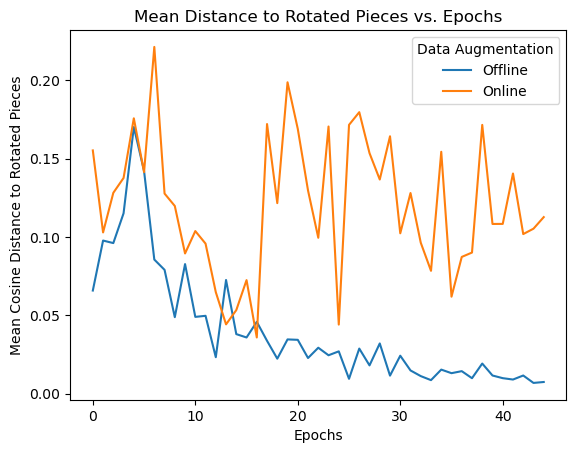
\includegraphics[width=\columnwidth]{images/mean_rotated_data_augmentation_type.png}
        \caption{Mean distance to rotated distribution.}
        \label{fig:mean_rotated_data_augmentation_type}
    \end{subfigure}
    \hfill
    \begin{subfigure}[h]{0.5\linewidth}
        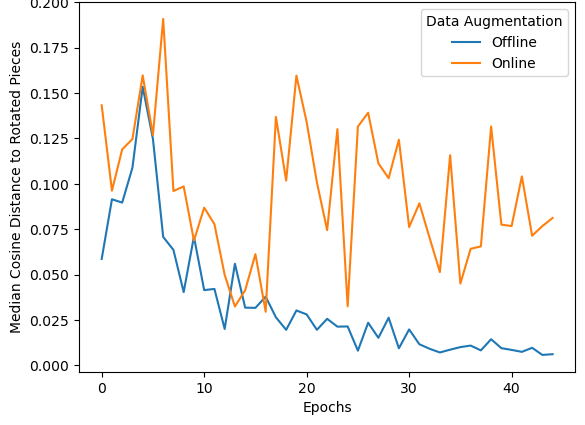
\includegraphics[width=\columnwidth]{images/median_rotated_data_augmentation_type.png}
        \caption{Median distance to rotated distribution.}
        \label{fig:median_rotated_data_augmentation_type}
    \end{subfigure}
    \caption{Influence of the type of data augmentation on the rotations metrics.}
    \label{fig:augmented_data_comparison}
\end{figure}

\subsection{Triplets metrics} 
\label{sec:triplet-metrics}

Training a triplet loss model is notoriously difficult. To better monitor the training process, several metrics were defined:
\begin{itemize}
    \item \textbf{Train easy triplets proportion}: This metric computes the proportion of easy triplets in the training set. An easy triplet results in a loss of 0.
    \item \textbf{Test easy triplets proportion}: This metric computes the proportion of easy triplets in the test set. 
    \item \textbf{Training triplets order}: This metrics computes the proportion of triplets that are 'correctly' ordered. A triplet is correctly ordered if the distance between the anchor and positive is less than the distance between the anchor and negative. This is the same as an easy triplet proportion for a triplet loss with margin 0.
    \item \textbf{Original triplets order}: This metrics computes the proportion of triplets that are 'correctly' ordered in the original dataset. It is important to notice here that these triplets do not belong to the training triplets, because the training triplets are augmented with random rotations.
\end{itemize}

Proportions of the training data were incorporated to analyze the model's behavior when converging to a loss of 0. The order of triplets was included to both assess the impact of the margin on triplet loss and to align with the fact that this order ultimately matters, as it's the one used by app users for labeling.

In addition to these metrics, we also computed the accuracy of the model on the small labeled dataset by evaluating the proportion of designs which nearest neighbor shares the same label. This metric is referred to as the \textbf{test accuracy}. We had to keep in mind that this accuracy gives a biased view of the model's performance, as the labeled dataset is not representative of the whole dataset.

We had also a heavy use of the interface to validate the model's performance qualitatively. Indeed better metrics do not always correlate with better real performance as it is shown in \autoref{sec:transformer-based-models}.

\section{Graph-based models}

Our original architecture involved a GNN model based on EdgeConv \cite{wangDynamicGraphCNN2019} convolution layers along with max pooling layers. 

Different convolution layers were tested for our backbone encoder, including Pointnet \cite{qiPointNetDeepHierarchical2017}, FeaStConv \cite{vermaFeaStNetFeatureSteeredGraph2018}, and PointTransformerConv \cite{zhaoPointTransformer2021}. The EdgeConv model was chosen as it yielded the best results.


On the one hand, EdgeConv operates on each node's local neighborhood, computing feature transformations for connected edges and aggregating this information. This captures local graph structure and node relationships. 

The max pooling layer then aggregates information across all nodes, creating a fixed-size graph representation that is invariant to the number of nodes and their ordering.
Given a graph with $N$ nodes, $F$ features and a feature matrix $X$ ($N$ rows, $F$ columns), global max pooling pools this graph into a single node is just one step. To compute the feature vector of this pooled node, it takes the feature-wise maximum across the node dimension of the graph. In other words, global max pooling finds for each feature/column in $X$ the node with the highest value and then takes this value into the pooled node vector. 

This combination allows the model to learn both local and global graph features effectively. The model works well because it can capture complex relationships in graph data, is scalable to different graph sizes, and learns hierarchical representations through stacked layers.

Here are a few key learnings we gathered along the way:

\paragraph{Use batch normalization}

Batch normalization \cite{ioffeBatchNormalizationAccelerating2015} turns out to be a crucial component for training our model. Not only does it speed up the training process, but it also improves the model's performance. This is particularly true for a similarity model, where the model must learn to differentiate between designs based on their cosine similarity. Dropout was also used in order to prevent overfitting.

\paragraph{Use large batch sizes}

Batching graph data is challenging because the number of nodes in each graph can vary. A dynamic batching strategy was implemented to handle this issue, fixing a maximum number of nodes per graph.
The size of the batch has a real impact on the model's performance. A larger batch size allows the model to learn more effectively, as it allows a greater triplets diversity within a single batch. We particularly observed this significance due to a change in the mesher for company-related reasons. Indeed, switching from Gmsh \cite{GmshThreedimensionalFinite} to BRepMesh\_IncrementalMesh \cite{BRepMesh_IncrementalMeshClassReference} led to different mesh sizes and configurations. The meshes generated from the BRepMesh were more complex, which reduced inevitably the batch size during training. We experienced a drop in the model's performance, but still good results. This shows the relative flexibility of such a model to adapt to different mesh format. This experience motivated us to explore the use of point clouds methods, such as the transformer-based model. These are more flexible because a uniform sampling can be applied to any mesh.

\paragraph{Insights into the triplet loss}

Triplet loss is notoriously difficult to train. Both the distance function and the margin can have a significant impact on the model's performance. The euclidean distance, notably used in FaceNet \cite{schroffFaceNetUnifiedEmbedding2015}, was tested but ultimately discarded in favor of the cosine similarity. The cosine similarity tends to be more robust to rotation changes, which is crucial for our model. The margin was set to 0.5, as it yielded the best results.

We soon encountered the problem of the loss rapidly converging to 0. It's why we added the triplets metrics introduced in \autoref{sec:triplet-metrics} to better monitor the training process.
Despite the loss trending towards zero, the classification accuracy began to decline just a few epochs after reaching peak values.
It became evident that many of the triplets were quickly classified as 'easy triplets' by the network. At this juncture, it was unclear whether the subsequent training performance was affected by the model architecture or the training loop itself.

To address the issue, in addition to adjusting the learning rates and dropout parameters, we implemented online triplets filtering within each batch, in order not to take into account certain type of triplets within the reduction. Indeed, the loss is rapidly converging to 0 because most of the elements within the reduction equal to 0.


In order of their performance:
\begin{enumerate}
    \item \textbf{Hard + Semi-Hard triplets filtering}: This approach involves only keeping the hard and semi-hard triplets. 
    \item \textbf{Semi-Hard triplets filtering}: This approach involves only keeping the semi-hard triplets.
    \item \textbf{Hard triplets filtering}: This approach involves only keeping the hard triplets.
\end{enumerate}

Since we are working in an unsupervised setting, it is not possible to generate triplets on the fly, like is suggested in \cite{moindrotTripletLossOnline2018}. Also, triplets that are classified as easy triplets at a given epoch can't just be discarded from the training set, as they might become hard triplets at a later epoch.


\label{sec:graph-based-models}
\begin{figure}[]
    \centering
    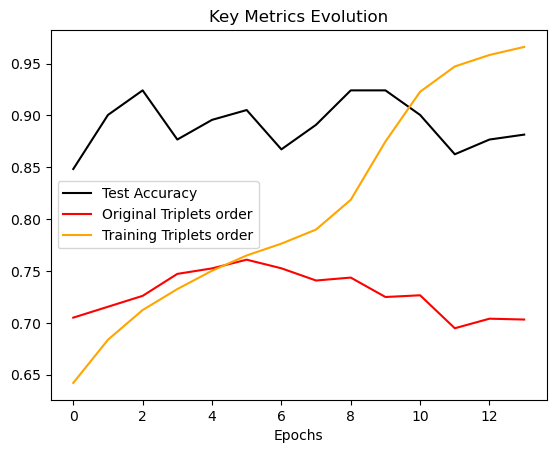
\includegraphics[width=0.5\columnwidth]{images/key_metrics_evolution_gnn.png}
    \caption{GNN model key metrics accuracies.}
    \label{fig:key_metrics_evolution_gnn}
\end{figure}

As shown in \autoref{fig:key_metrics_evolution_gnn}, the model quickly reaches a great accuracy on the test set. However, the original triplets order metrics starts decreasing after a few epochs, even if the loss continues to decrease. This shows the limitations of this architecture, as it is not able to further learn the correct order of the triplets. This tendency will be fixed by using a transformer-based model.


\section{Transformer-based models}
\label{sec:transformer-based-models}

As explained previously, several points made us pivot towards point cloud transformer models.
\begin{itemize}
    \item Growing popularity of point cloud transformer models in the field of 3D data processing.
    \item Flexibility of point cloud models. They are less dependent on the input mesh format, as a uniform sampling can be applied to any mesh.
    \item Easy switch from a mesh to a point cloud format.
\end{itemize}

The goal was to study the performance of a pre-trained encoding model our on data, as well as a fine-tuned model with our triplets. Several backbones were tested, such as ReCon++ \cite{qiShapeLLMUniversal3D2024} or PointTransformer \cite{zhaoPointTransformer2021}. The best results were obtained with the OpenShape model \cite{liuOpenShapeScaling3D2023}. Indeed, the pre-trained model already showed improved performance in comparison with our best GNN model, as it can be seen from the starting performance in \autoref{fig:key_metrics_evolution_openshape}. The fine-tuned model was able to reach even better results, as shown in \autoref{fig:key_metrics_evolution_openshape}.

We can clearly see the increasing metrics as the loss decreases, which was clearly not the case with the GNN model. The model is able to learn the correct order of the triplets, as shown by the original triplets order metrics. The rotation metrics are also improving, as shown in \autoref{fig:rotation_metrics_evolution_openshape}.
This highlights the remarkable ability of transformers architectures to learn intricate patterns in the data, regardless of its nature.

\begin{figure}[]
    \centering
    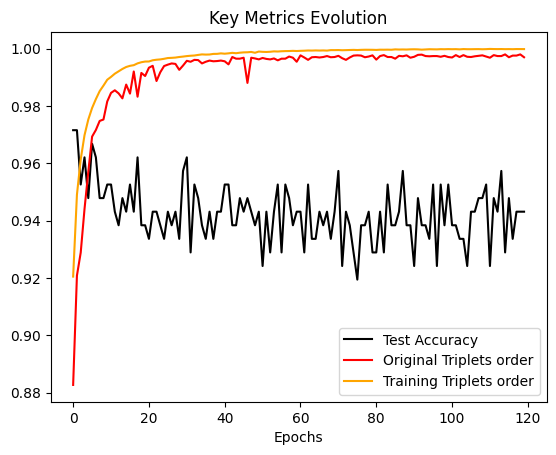
\includegraphics[width=0.5\columnwidth]{images/key_metrics_evolution_openshape.png}
    \caption{Fine-tuned model key metrics accuracies.}
    \label{fig:key_metrics_evolution_openshape}
\end{figure}

\begin{figure}[]
    \begin{subfigure}[h]{0.5\linewidth}
        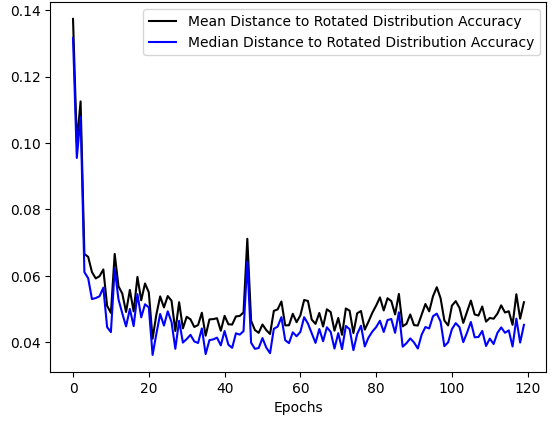
\includegraphics[width=\columnwidth]{images/rotation_metrics_evolution_openshape.png}
        \caption{Distances to rotated designs accuracies.}
    \end{subfigure}
    \hfill
    \begin{subfigure}[h]{0.5\linewidth}
        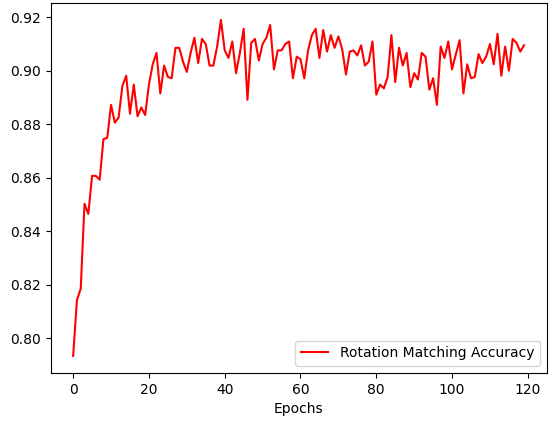
\includegraphics[width=\columnwidth]{images/rotation_accuracy_evolution_openshape.png}
        \caption{Rotation matching accuracy.}
    \end{subfigure}
    \caption{Fine-tuned model rotation accuracies.}
    \label{fig:rotation_metrics_evolution_openshape}
\end{figure}

As a final benchmark, we compared in the interface the nearest neighbors of a design given by the transformer pre-trained model and by the fine-tuned model. Even if fine-tuned model is better in terms of metrics, the qualitative results are not always better. This shows the limitations of the metrics and the importance of the interface to validate the final model's performance, especially in our unsupervised setting.
%%% Local Variables: 
%%% mode: latex
%%% TeX-master: "isae-report-template"
%%% End: 